\documentclass{homework}
\usepackage{lipsum}
\usepackage{cancel}
\usepackage{amsthm}
\usepackage{cleveref}
\usepackage{upgreek}
\usepackage{mathrsfs}
\usepackage{tikz}
\usepackage{units}
\newtheorem{lemma}{Lemma}

\DeclareMathOperator{\cov}{cov}

\title{Kevin Joyce}
\course{Stat 542 - Applied Linear Models - Homework 2}
\author{Kevin Joyce}
\docdate{\today}
\begin{document} 
\newcommand{\figref}[1]{\figurename~\ref{#1}}
\renewcommand{\bar}{\overline}
\renewcommand{\hat}{\widehat}
\renewcommand{\SS}{\mathcal S}
\newcommand{\HH}{\mathscr H}
\newcommand{\mom}{\widetilde}
\newcommand{\mle}{\widehat \Uptheta}
\newcommand{\eps}{\varepsilon}
\newcommand{\todist}{\stackrel{D}\longrightarrow}
\newcommand{\toprob}{\stackrel{p}\longrightarrow}
\newcommand{\TTheta}{\overline{\underline \Theta} }
\newcommand{\del}{\partial}
\newcommand{\approxsim}{\overset{\cdotp}{\underset{\cdotp}{\sim}}}
\begin{longproblem}
  Faraway 2.1. The dataset \texttt{teengamb} concerns a study of teenage gambling in Britain.  Fit a regression model with the expenditure on gambling as the response and the sex, status, income and verbal score as predictors.  Present the output.
\begin{verbatim}
Call:
lm(formula = gamble ~ sex + status + income + verbal)

Residuals:
    Min      1Q  Median      3Q     Max 
-51.082 -11.320  -1.451   9.452  94.252 

Coefficients:
             Estimate Std. Error t value Pr(>|t|)    
(Intercept)  22.55565   17.19680   1.312   0.1968    
sex         -22.11833    8.21111  -2.694   0.0101 *  
status        0.05223    0.28111   0.186   0.8535    
income        4.96198    1.02539   4.839 1.79e-05 ***
verbal       -2.95949    2.17215  -1.362   0.1803    
---
Signif. codes:  0 ‘***’ 0.l standard error: 22.69 on 42 degrees of freedom
Multiple R-squared: 0.5267,     Adjusted R-squared: 0.4816 
F-statistic: 11.69 on 4 and 42 DF,  p-value: 1.815e-06 

\end{verbatim}

  \subproblem{ What percentage of variation in the response is explained by these predictors? }

This is given by $R^2$, i.e.~\unit[53]{\%}.

  \subproblem{ Which observation has the largest (positive) residual?  Give the case number. }

The 39th indexed response has the minimum residual of $-51.082$. 

  \subproblem{ Compute the mean and median of the residuals. }

Theoretically we expect that the mean residual is $0$.  When calculated it, is $ < 3\times 10^{-16}$. The median residual is  $-1.451$, indicating right skewness in the residual distribution.

  \subproblem{ Compute the correlation of the residuals with the fitted values. }

Assuming homogeneity of variance, we expect this to be $0$, and, when calculated, it is $< 3\times 10^{-17}$.

  \subproblem{ Compute the correlation of the residuals with the income.  }

This quantity was computed to be less than $6\times 10^{-17}$, again expected to be 0 when the assumption of homogeneity is met. 

  \subproblem{ For all other predictors held constant, what would be the difference in predicted expenditure on gambling for the male compared to a female? }

  This is given by the coefficient corresponding to \texttt{sex}.  Since $0$ was coded for males, we expect that males gamble \unit[22.12]{\pounds} more a week than females on average when all other explanatory variables are held constant.
\end{longproblem}
\newpage

\begin{longproblem}
  Faraway 2.3. In this question, we investigate the relative merits of methods for computing the coefficients.  Generate some artificial data by:
\begin{verbatim}
> x <- 1:20
> y <- x+rnorm(20)
\end{verbatim} 
Fit a polynomial in \texttt{x} for predicting \texttt y.  Compute $\hat \beta$ in two ways -- by \texttt{lm()} and by using the direct calculation described in the chapter.  At what degree of polynomial does the direct calculation method fail?  (Note the need for the \texttt{I()} function in fitting the polynomial, that is, \verb|lm(y ~ x + I(x^2))|.
\end{longproblem}
\begin{solution}
  Rather than following Faraway's suggestion, we employ the function \texttt{vandermonde.matrix} in the \texttt{matrixcalc} library.  E.g.~a design matrix for a quadratic model on \texttt{x = c(1,2,3,4,5)} is given by
\begin{verbatim}
> vandermonde.matrix(1:5,3)
     [,1] [,2] [,3]
[1,]    1    1    1
[2,]    1    2    4
[3,]    1    3    9
[4,]    1    4   16
[5,]    1    5   25
\end{verbatim}
We can now easily loop through the possible design matrices given by: 
\begin{verbatim} A = vandermonde.matrix(x,20) \end{verbatim} The results follow:
\begin{verbatim}
> for (i in 2:20) { print(solve(crossprod(A[,1:i],A[,1:i]),crossprod(A[,1:i],y))) }
           [,1]
[1,] -0.2054614
[2,]  1.0541753
             [,1]
[1,] -0.564601934
[2,]  1.152122725
[3,] -0.004664162

... % OUTPUT OMITTED

              [,1]
[1,] -8.717609e-01
[2,]  1.602359e+00
[3,] -1.733619e-01
[4,]  2.380631e-02
[5,] -1.394025e-03
[6,]  2.864698e-05
Error in solve.default(crossprod(A[, 1:i], A[, 1:i]), crossprod(A[, 1:i],  : 
  system is computationally singular: reciprocal condition number = 3.54243e-18

\end{verbatim}
Hence, solving the normal equations is only numerically possible for up to fifth degree polynomials, and the design matrix will necessarily have two columns that are ``numerically linearly dependent'' in the sense that $A^TA$ will be numerically singular.

Using \texttt{lm( ... )} seems to use a more stable method as a full list of parameters are reported up to 13th degree polynomials.
\begin{verbatim}
> A = A[,-1] % remove intercept column
> for (i in 1:19) { # This will use lm( ... ) to find the parameters
+   out = lm(y ~ A[,1:i])
+   print(sprintf("--------------- i = %d -------------",i))
+   print(summary(out))
+ } 

... % OUTPUT OMITTED

[1] "--------------- i = 13 -------------"

Call:
lm(formula = y ~ A[, 1:i])

Residuals:
     Min       1Q   Median       3Q      Max 
-1.53293 -0.21569  0.02872  0.24767  1.43972 

Coefficients: (1 not defined because of singularities)
              Estimate Std. Error t value Pr(>|t|)
(Intercept) -1.899e+01  1.009e+02  -0.188    0.856
A[, 1:i]1    3.506e+01  2.576e+02   0.136    0.896
A[, 1:i]2   -1.816e+01  2.598e+02  -0.070    0.946
A[, 1:i]3    8.977e-01  1.409e+02   0.006    0.995
A[, 1:i]4    2.516e+00  4.672e+01   0.054    0.959
A[, 1:i]5   -1.098e+00  1.012e+01  -0.108    0.917
A[, 1:i]6    2.332e-01  1.489e+00   0.157    0.880
A[, 1:i]7   -2.996e-02  1.511e-01  -0.198    0.849
A[, 1:i]8    2.473e-03  1.059e-02   0.233    0.822
A[, 1:i]9   -1.322e-04  5.032e-04  -0.263    0.800
A[, 1:i]10   4.434e-06  1.546e-05   0.287    0.782
A[, 1:i]11  -8.481e-08  2.769e-07  -0.306    0.768
A[, 1:i]12   7.063e-10  2.196e-09   0.322    0.757
A[, 1:i]13          NA         NA      NA       NA

... % OUTPUT OMITTED
\end{verbatim}

\end{solution}
\newpage

\begin{longproblem}
  Faraway 2.4. The dataset \texttt{prostate} comes from a study on 97 men with
  prostate cancer who were due to receive a radical prostatectomy.  Fit a model
  with \texttt{lpsa} as the response and \texttt{lcavol} as the predictor.
  Record the residual standard error and the $R^2$.  Now add
  \texttt{lweight,svi,lpbh,age,lcp,pgg45} and \texttt{gleason} to the model one
  at a time.  For each model record the residual standard error and the $R^2$.
  Plot the trends in these two statistics.
\end{longproblem}

\begin{solution}
For \verb|lpsa ~ lcavol|, the calclated $R^2$ is 0.5394 and the residual standard error is 58.915.

In the following table we add \texttt{lweight,svi,lpbh,age,lcp,pgg45} and \texttt{gleason} to the model in order
and record the resulting $R^2$ and RSS.

\begin{minipage}{.48\textwidth}
\begin{tabular}{l | c c}
\hline
Explanatory Variables & $R^2$ & RSS \\ \hline
\texttt{lcavol} &      0.539 & 58.91 \\
\texttt{...+lweight} & 0.586 & 52.97 \\
\texttt{...+svi} &     0.626 & 47.78 \\
\texttt{...+lpbh} &    0.637 & 46.48 \\
\texttt{...+age} &     0.644 & 45.53 \\
\texttt{...+lcp} &     0.645 & 45.40 \\
\texttt{...+pgg45} &   0.654 & 44.20 \\
\texttt{...+gleason} & 0.655 & 44.16 \\
\hline
\end{tabular}
\end{minipage}
\begin{minipage}{.48\textwidth}
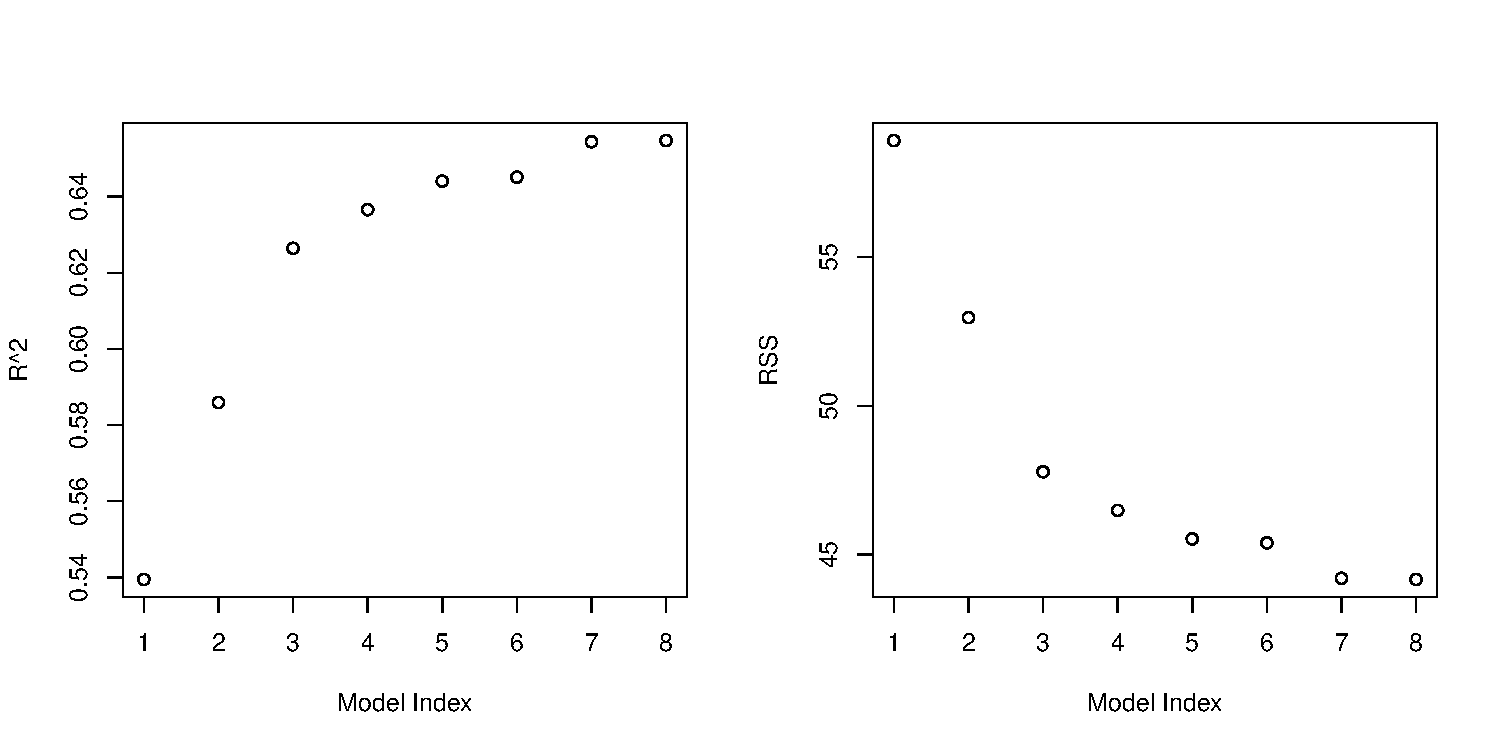
\includegraphics[width=\textwidth]{parameter_add_trends.pdf}
\end{minipage}

Note that as explanatory variables are added, the model predictive
power ($R^2$) increases and that the distance from the predictions
to the data (the residual sums of squares) decreases as expected.  The trends are non-linear, and indicate ``diminishing returns'' in the sense that adding an additional parameters reduces the RSS and increases $R^2$ less and less.  
\end{solution}

\begin{longproblem}
  Faraway 2.5. Using the \texttt{prostate} data, plot \texttt{lpsa} against \texttt{lcalvol}.  Fit the regression of \texttt{lpsa} on \texttt{lcavol} and \texttt{lcavol} on \texttt{lpsa}.  Display both regression lines on the plot.  At what point do the two lines intersect?
\end{longproblem}

\begin{solution}
\begin{minipage}{.45\textwidth}
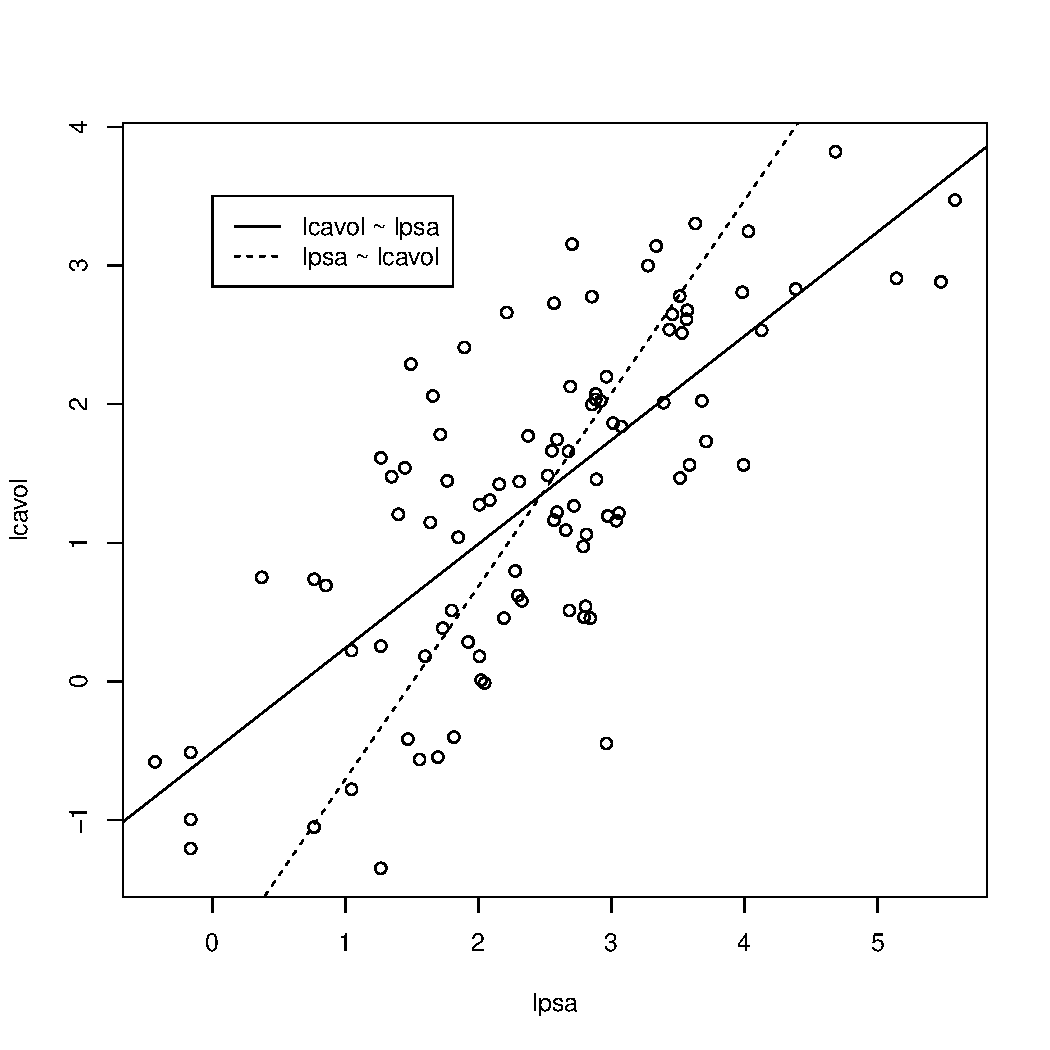
\includegraphics[width=\textwidth]{two_lines.pdf}
\end{minipage}
\begin{minipage}{.45\textwidth}
  Note that the least squares line for \verb|lcavol ~ lpsa|
  minimizes the vertical distance from the lines to the points, and
  the least squares line for \verb|lpsa ~ lcavol| minimizes the
  horizontal distance.  Hence, their intersection occurs at the
  respective means,
  i.e.~at $(\bar{\mathtt{lpsa}},\bar{\mathtt{lcavol}}) = (2.478, 1.350)$
\end{minipage}

\end{solution}

\begin{longproblem}
  In an industrial laboratory, under uniform conditions, batches of electrical insulating fluid were subjected to constant voltages until the insulating property of the fluids broke down.  Seven different voltage levels, spaced 2 kilovolts (kV) apart from 26 to 38 kV, were studied.  The measured responses were the time, in minutes, until breakdown.  These data can be found on the course webpage under the file \texttt{fluid.txt}.  [Data from W.B. Nelson, Schenectady, NY: GE Co. Tech. Report 71-C-011 (1970).]

\subproblem{ Construct a scatterplot of breakdown time vs. voltage and describe the association.  Can you suggest a nonlinear model that could be fit to these data?  IF you were to fit such a model, would the homogeneous error variance assumption be valid?}

\begin{minipage}{.45\textwidth}
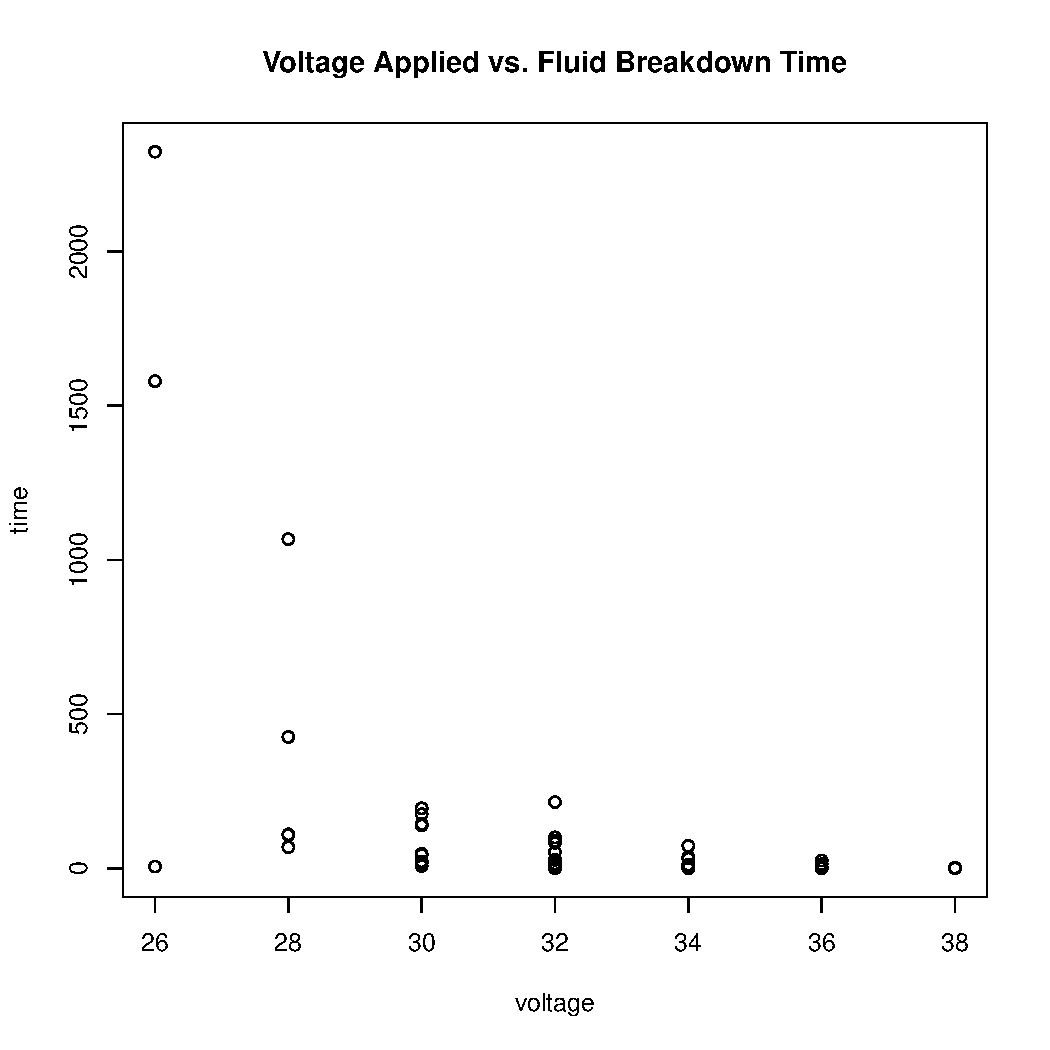
\includegraphics[width=\textwidth]{voltage_time_scatter.pdf}
\end{minipage}
\begin{minipage}{.45\textwidth}
Perhaps a reciprocal model is appropriate in this case, i.e. the response time $y_i$ is modeled by the reciprocal voltage $1/x_i$. This would require that a fluid have an arbitrarily long breakdown time for no applied voltage.  Although, since the response is not a ratio, this may not make sense.  Note that any curve that fits this model will \emph{not} have homogeneous additive error.
\end{minipage}

\subproblem{ As mentioned in class, transformation on variables are performed for many reasons.  In a regression setting, in addition to linearizing the relationship between two variables, transformations sometimes will correct violations of other model assumptions, such as the error variance homogeneity assumption.  Take the (natural) log of the breakdown times, plot these against the voltages, and describe the resulting association between the variables.  Discuss whether this transformation also homogenized the error variance.}

\begin{minipage}{.4\textwidth}
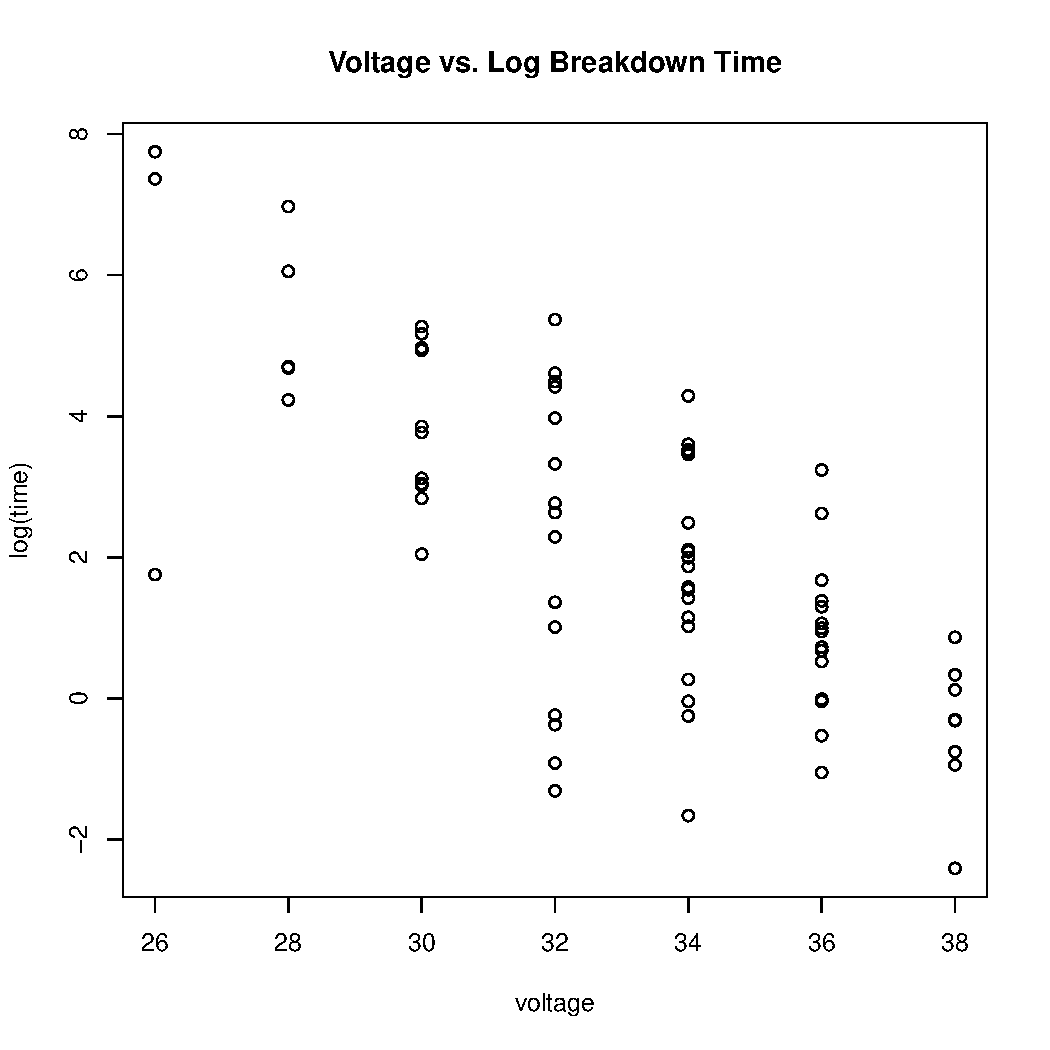
\includegraphics[width=.95\textwidth]{voltage_logtime.pdf}
\end{minipage}
\begin{minipage}{.45\textwidth}
It appears that log transforming the breakdown time response results in a nearly linear negative association with voltage.  The issues with variance homogeneity are much better, but not perfect.  That is, there appears to be more variation for higher voltages.
\end{minipage}
\newpage

\subproblem{ Fit the simple linear regression model with log(breakdown time) as the response and voltage as the explanatory variable, and report the regression equation.  What breakdown time is predicted for a voltage of \unit[35]{kV}?}

The least squares solution for fitting 
\begin{equation}
  \log y_i = \beta_0 + \beta_1 x_i + \epsilon_i\label{logmodel}
\end{equation}
results in $\hat{\beta_0} \approx18.96$ and $\hat{\beta_1}\approx0.507$. 

\subproblem{ Give an interpretation of the slope in terms of the voltages and the raw breakdown times. In other words, don't interpret the slope in terms of the log breakdown times. }

Since the raw breakdown time is given by $e^{\beta_0}e^{\beta_1 x_i}e^{\epsilon_i}$, we have with each unit increase in voltage, the predicted breakdown time is reduced by a factor of $e^{\hat{\beta_1}} \approx 0.602$, or reduced by approximately \unit[40]{\%}.

\subproblem{ Compute and interpret the coefficient of determination $R^2$. }

The computed $R^2$ is 0.514, so about \unit[51]{\%} of the variation in the \emph{log} breakdown time is explained by the model in \eqref{logmodel}.

\subproblem{ Construct a residual plot and normal quantile plot on the residuals for this model and explain what the plots indicate about the regression model. }

\begin{minipage}{.35\textwidth}
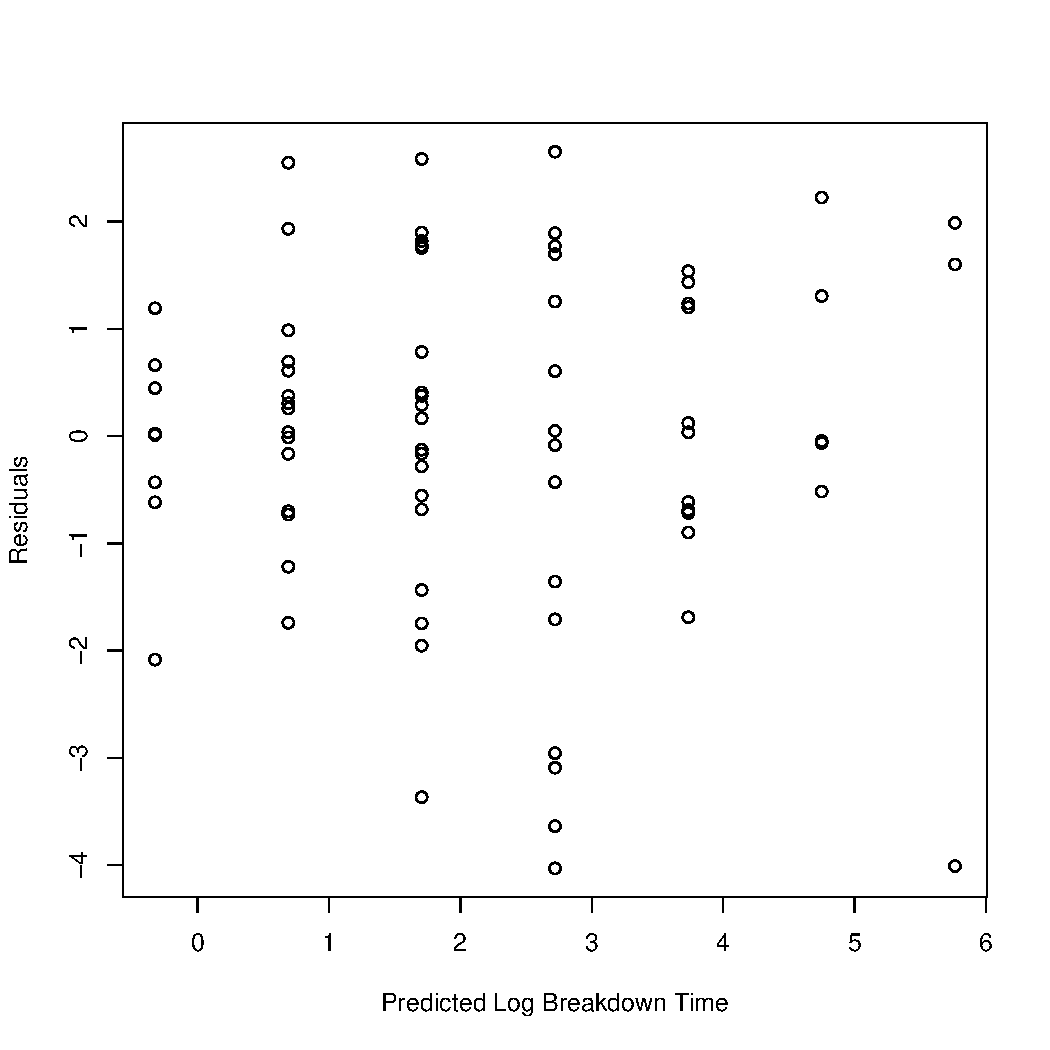
\includegraphics[width=\textwidth]{residual_fluid.pdf}
\end{minipage}
\begin{minipage}{.55\textwidth}
There appears to be no exceptionally noticable patterns in the residual plot.  The point in the lower left corner corresponds to the over-predicted point measured at 26 Volts.  If this point were removed, there may be an argument for non-homogeneous variance. 
\end{minipage}

\begin{minipage}{.35\textwidth}
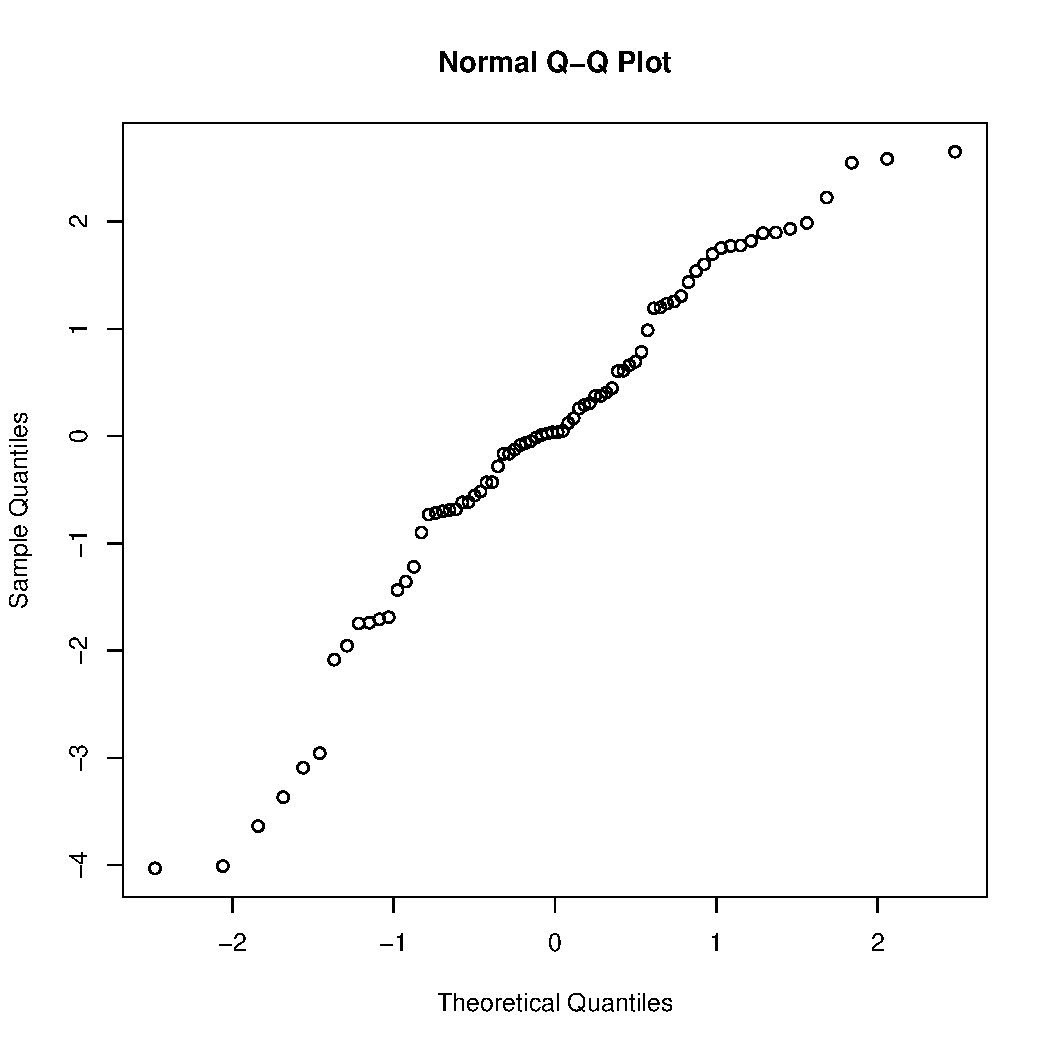
\includegraphics[width=\textwidth]{qqplot_fluid.pdf}
\end{minipage}
\begin{minipage}{.55\textwidth}
The general linearity of the qqplot to the left suggests that the assumption of normality of the residuals may be reasonable, although the lower points in the left tail indicate that the residuals may be left skewed and the lower points on the right tail may indicate that the distribution does not ``spread to the right'' enough.  The Shapiro-Francia test gives $p = 0.0197$, giving some evidence of non-normality.
\end{minipage}

\subproblem{ Suppose in addition to these two variables, a third variable (let's just call it temperature, even though I completely made it up!) is measured in this experiment, as given in the 3rd column of the data set.  Fit a linear regression model with log(breakdown time) as the response and voltage \& temperature as explanatory variables.  Report the ANOVA table for this regression fit and explain in a few sentences what is happening with this model.}

We report the output of \texttt{summary(lm(log(time) = voltage + temp))}.
\begin{verbatim}
Residuals:
    Min      1Q  Median      3Q     Max 
-3.9963 -0.7736  0.0380  1.1381  2.8661 

Coefficients:
            Estimate Std. Error t value Pr(>|t|)    
(Intercept)  15.1988     4.1930   3.625 0.000532 ***
voltage      -0.3230     0.1919  -1.683 0.096617 .  
temp         -0.1745     0.1734  -1.006 0.317554    
---
Signdard error: 1.56 on 73 degrees of freedom
Multiple R-squared: 0.5203,     Adjusted R-squared: 0.5071 
F-statistic: 39.58 on 2 and 73 DF,  p-value: 2.273e-12 
\end{verbatim}

In this model, note that the voltage coefficient is no longer
significant, whereas, without temperature added, the $p$-value was less than $4\times10^{13}$.
Comparison between the significance of these two parameters is not meaningful
unless we consider them in the context of the model that the parameters are in.
That is, adding temperature (which may not even have an effect on breakdown time) to the model
 had the effect that the voltage coefficient is now less significant in our \emph{new model's predicted} log breakdown time
for each unit voltage increase. 
\end{longproblem}

\problem{The 1994 World Almanac reports heights and numbers of stories for notable tall buildings in North America.  A random sample of 60 buildings among those in the list for which dates a completion were available was taken.  The data appear under the filename \texttt{building.txt} on the course web page in four columns.  The columns in order consist of the building name, year of completion, height (feet), and number of stories. Analyze the data and write a brief statistical report including a summary of statistical findings and any relevant graphical displays, where you address the following questions.  What is the distribution of the number of stories as a function of height?  What is the mean height per story?  Are there any buildings that have particularly fewer stories than expected for their height?  Are there any buildings that have particularly more stories  than expected for their height?  Is there any indication that the number of stories per height has changed over the time period represented here?}

\begin{solution}
\begin{minipage}{.3\textwidth}
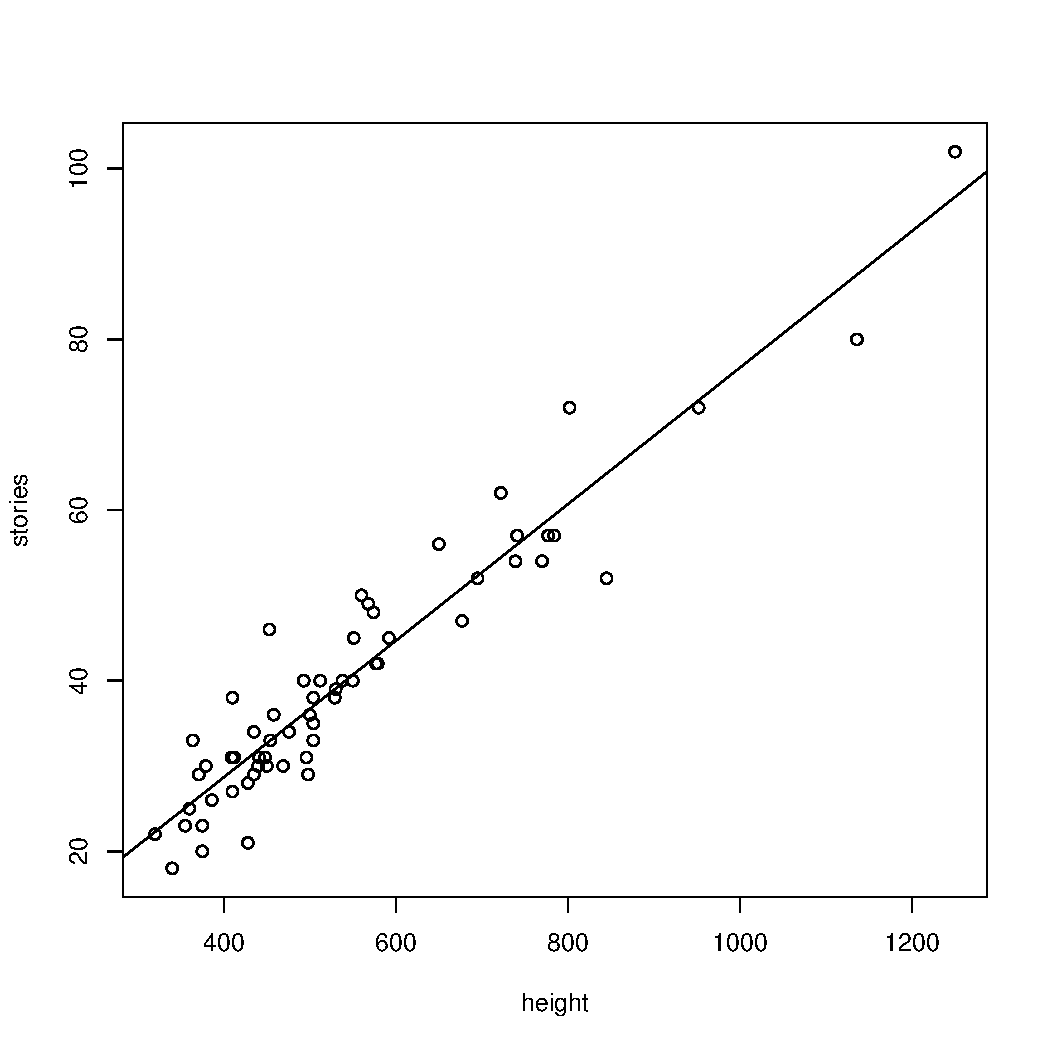
\includegraphics[width=\textwidth]{height_vs_stories.pdf}
\end{minipage}
\begin{minipage}{.6\textwidth}
To the left, we've plotted the building stories vs.~height with a least-squares
line.  Plotting stories versus height indicates a strong positive linear
association.  Variance appears to be homogeneous along the line.  An estimate
for the mean height increase per story is given by the slope of least squares
line that predicts height by stories, which is $\hat \beta_1 =$
\unit[11.29]{ft/story}.  Based on the apparent lack of outliers in the plot,
there are no are no buildings with more or less stories than expected.
Both the qqplot and residuals plot indicate no lack of assumption issues
with either linear model.
\end{minipage}

\begin{minipage}{.4\textwidth}
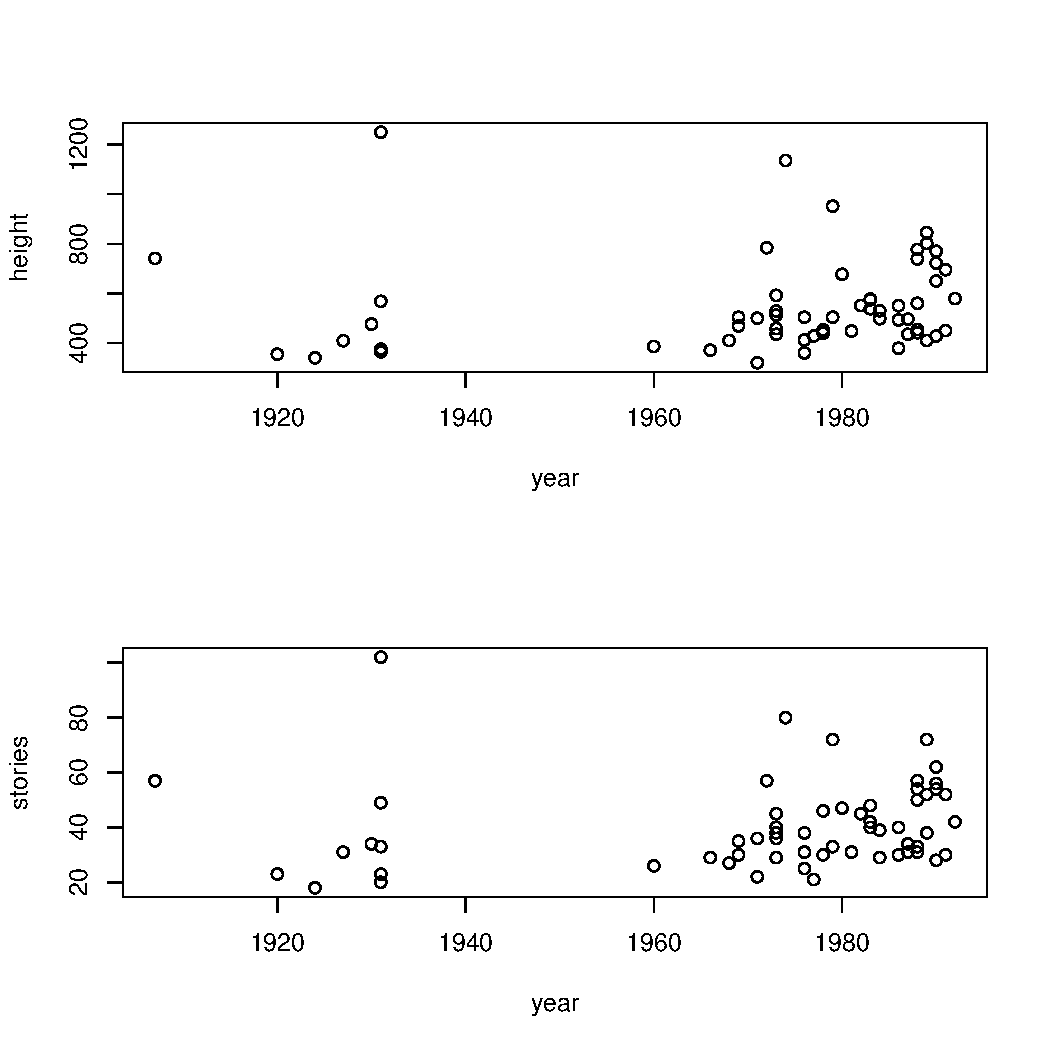
\includegraphics[width=.8\textwidth]{building_timeseries.pdf}
\end{minipage}
\begin{minipage}{.5\textwidth}
We first note that plots of both height and stories versus year indicate a lack
of data from 1930 to 1960 which may indicate that some set of events may have
prevented or greatly inhibited the construction of notable tall buildings in
that time period.  Moreover, it suggests that we may want to consider buildings
prior to 1930 and those built after 1960 separate populations or include this
as an indicator variable in the model.
\end{minipage}
If we separately estimate the mean change in height per story in these two
populations, we obtain for pre-1930 buildings $\hat \beta_1 = 10.97$ with
standard error $0.687$ and $\hat \beta_1' = 11.5$ with standard error $0.648$.
By no means a formal test, this does indicate that there may be a some
difference in the mean height per story between these two time periods.
\end{solution}
\newpage

\problem{ For the simple linear regression model ($y_i = \beta_0 + \beta_1 x_i
+ \epsilon_i$), show that $\mathrm{Cov}(\bar y, \hat{\beta}_1)=0$ whenever
$\mathrm{Var}(\epsilon_i) = \sigma^2$ for all $i$ and
$\mathrm{Cov}(\epsilon_i,\epsilon_j) = 0$ for all $i\not=j$.}

\begin{solution}
  Using a result from calculating the variance of $\beta_1$ in the notes and bilinear properties of covariance, we have
  \begin{align*}
  \cov(\bar y, \hat \beta_1) 
  &= \cov\left(\frac 1n \sum_{i=1} y_i, \frac 1{s_{xx}} \sum_{j=1}^n(x_j - \bar x)y_j\right) \\
  &= \frac 1n \sum_{i=1}^n \sum_{j=1}^n (x_j-\bar x) \cov(y_i,y_j)\\
  &= \frac 1n \sum_{i=1}^n \sum_{j=1}^n (x_j-\bar x) \cov(\epsilon_i,\epsilon_j)\quad\text{ since }y_i = \beta_0 +\beta_1 x_i + \epsilon_i\\
  &= \frac 1n \sum_{i=1}^n (x_i - \bar x) \sigma^2 = 0\quad\text{ since } \cov( \epsilon_i = \epsilon_j ) = 0\text{ for }i\not=j\text{ and sums of residuals are 0.}\\
  \end{align*}
\end{solution}

\problem{Prove the last equality on page 51 of the class notes for the MSE, namely that:
$$
  \mathrm{MSE} = \frac 1{n-2} \Big[(n-1)s_y^2 - \hat\beta_1^2(n-1)s_x^2\Big].
$$}

\begin{solution}
  Recall that $\hat \beta_0 = \bar y - \hat \beta_1 \bar x$ and $\hat \beta_1 = \frac{s_{xy}}{s_{xx}}$.  Continuing from page 51,
  \begin{align*}
    MSE &= \frac 1{n-2} \sum_{i=1}^n(y_i - \hat \beta_0 - \hat \beta_1 x_i)^2\\
    &= \frac1{n-2} \sum_{i=1}^n\Big( (y_i - \bar y) + \hat\beta_1(\bar x - x_i)\Big)^2\\
    &= \frac1{n-2} \sum_{i=1}^n\Big((y_i - \bar y)^2 - 2\hat\beta_1(y_i - \bar y)(x_i - \bar x) + \hat\beta_1^2(x_i - \bar x)^2 \Big)\\
    &= \frac1{n-2} \Big( (n-1)s_y^2 - 2\frac{s_{xy}}{s_{xx}}s_{xy} + \left(\frac{s_{xy}}{s_{xx}}\right)^2 s_{xx} \Big)\\
    &= \frac1{n-2} \Big( (n-1)s_y^2 - \hat \beta_1 (n-1)s_x^2 \Big).\\
  \end{align*}
\end{solution}
\end{document} 
